\documentclass[a4j,12pt]{jsarticle}
\usepackage{semi}
\begin{document}


\日付{2018/07/03}
\氏名{阿部 希駿}
\タイトル{卒業研究}

\semi

\section{緒言}
文部科学省が発表した国際学力調査によると世界の中でも日本の学力は上位にある.しかし日本の学生の学力は二極化していると言われ,問題点は多い.
二極化の下の山の学生は学習内容の一部がわからないのではなく,「何をしているのかがわからない」「どこがわからないのかもわからない」などという根本的な原因があると推測している.

また各塾の調査では中学,高校で学習する科目の中で数学と英語は苦手になりやすいと言われている.この2科目の共通点として既に学習した知識を使うことを前提として授業を行う積み上げ型教科という点がある.積み上げ型教科では単元の内容が複雑になるほど必要な前提知識が多くなり,どの単元の内容が使われているかがわかりにくくなる.そのためその単元の内容を理解をすることが難しくなることが問題点としてあげられる.

そこで「単元ごとの繋がりや,その単元を前提知識とする単元の概要をあらかじめ説明することで個々の単元の内容の理解を促進することができる」という仮説を立てた.
この仮説では特に複数の単元の学習内容を用いて学習を行う単元で,用いる単元の内容などの具体的なイメージがしづらい場合を対象にする.
本研究では,講義にて学生を対象にして実験を行い,この仮説を検証することを目的とする.
講義では「ブロックチェーン」を対象にする.学習の過程である「暗号」や「ハッシュ」の段階では計算などの学習がメインで目的がわかりづらいが,「ブロックチェーン」では


\section{教科の特性}
学校で学習する教科には独立型教科と積み上げ型教科に分かれ,それぞれ下図のように積み木のような図で表される.

\begin{figure}[H]
\centering
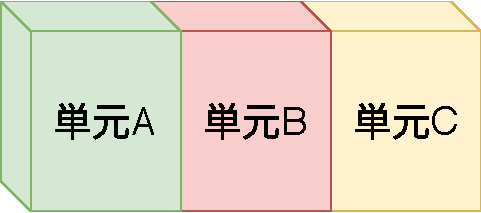
\includegraphics[width=7cm]{02.pdf}
\caption{独立型教科の教育モデル}
\label{fig:02}
\end{figure} 

\begin{figure}[H]
\centering
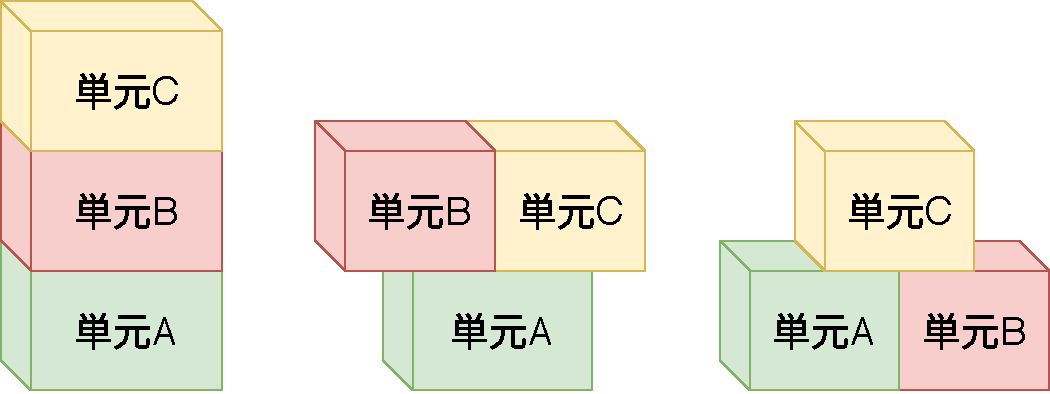
\includegraphics[width=12cm]{03.pdf}
\caption{積み上げ型教科の教育モデル}
\label{fig:03}
\end{figure} 

\subsection{独立型教科}
独立型教科は国語や社会が該当する.
独立型教科では図\ref{fig:01}のように各単元が独立していて関連性があまりないためどの単元から学習しても支障がない.
\begin{figure}[H]
\centering
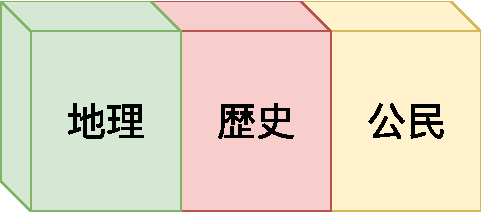
\includegraphics[width=6cm]{01.pdf}
\caption{独立型教科の例}
\label{fig:01}
\end{figure} 

\subsection{積み上げ型教科}
積み上げ型教科では数学や英語が該当する.
積み上げ型教科では図\ref{fig:04}のように学習した内容を次の学習の基礎知識として用いるため,順番に学習していくことになる.

\begin{figure}[H]
\centering
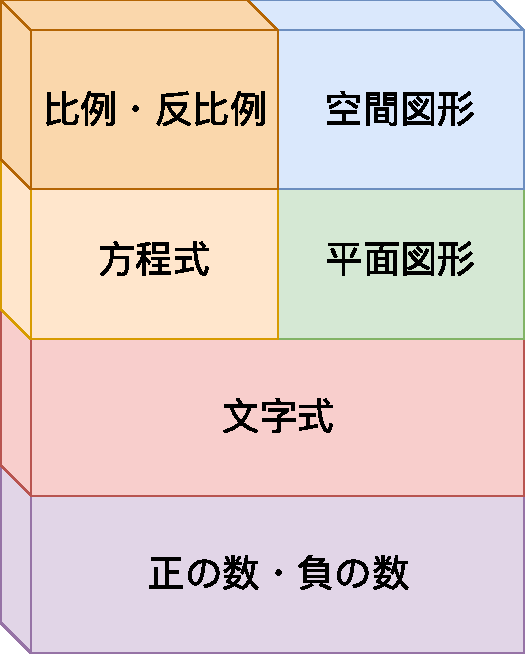
\includegraphics[width=5cm]{04.pdf}
\caption{積み上げ型教科の例}
\label{fig:04}
\end{figure} 

\section{暗号について}
暗号とは通信を行う際,第三者にその内容を知られないようにするための手段である.
元の文に一定の規則を用いて特定の変形を加えることを暗号化,暗号化する前の元の文を平文,暗号から平文に戻すことを復合化(復号)と呼ぶ.
暗号化する手段が暗号アルゴリズムであり,また暗号化や復号化に使うデータを鍵と呼ぶ.
暗号は特性によって古典暗号と現代暗号に分かれる.
アルゴリズムがわかれば解読が容易になる暗号を古典暗号,アルゴリズムは公開するが鍵を非公開にすれば安全な暗号を現代暗号という.

\subsection{共通鍵暗号}
暗号化と復号に同じ鍵を用いる暗号の方式である.


\subsubsection{換字式暗号の仕組みと例}
平文の文字を他の記号や文字に置き換えて暗号文を作る古典暗号の方式である.
換字式暗号の代表としてシーザー暗号がある.
シーザー暗号は鍵である決められた文字数分のアルファベットをずらして暗号化を行う.
図\ref{fig:05}は鍵が1であるときの例である.

\begin{figure}[H]
\centering
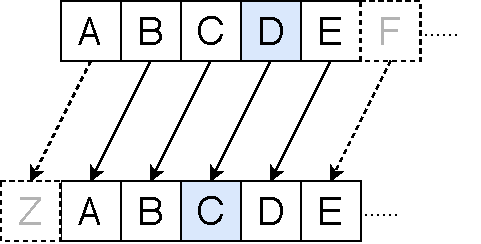
\includegraphics[width=9cm]{05.pdf}
\caption{シーザー暗号の例}
\label{fig:05}
\end{figure} 


\subsubsection{転置式暗号の仕組みと例}
平文の位置を並び替えて暗号文を作る古典暗号の方式である.
転置式暗号の代表としてスキュタレー暗号がある.
スキュタレー暗号はスキュタレーと呼ばれるシリンダーに細長い紙を巻きつけ,平文を横書きに書く.
紙をスキュタレーから外すと順番が入れ替わった暗号ができる.
暗号の受け取る側は同じ半径のスキュタレーを用意し,紙を巻きつけることで復号することができる.
この場合,鍵は同じ直径であることである.

\begin{figure}[H]
\centering
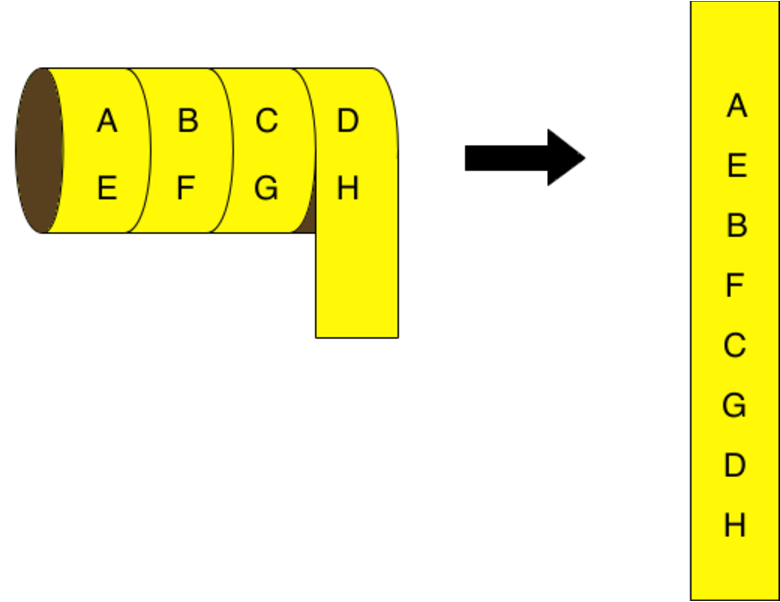
\includegraphics[width=9cm]{062.pdf}
\caption{スキュタレー暗号の例}
\label{fig:06}
\end{figure} 



\subsection{公開鍵暗号}
暗号化と復号に別の手順を用いる暗号方式である.

\subsubsection{RSA暗号の仕組みと例}
RSA暗号は桁数の多い素因数分解問題が困難であることを安全性の根拠とした公開鍵暗号の一つである.

\subsection{SSL暗号化通信}
SSL暗号化通信



\subsection{暗号の歴史}







\section{ハッシュについて}

\section{ブロックチェーンについて}

\section{実験}


\section{実験結果}

\section{考察}

\section{結言}

\section{参考文献}

\section{謝辞}

\section{付録}

\end{document}